\documentclass[tikz,border=4pt]{standalone}
\usepackage{amsmath,amssymb}
% Grupo Nostradamus - lenguaje visual TikZ
\definecolor{nostranavy}{HTML}{061426}
\definecolor{nostrateal}{HTML}{078C95}
\definecolor{nostracyan}{HTML}{65DCE5}
\definecolor{nostragold}{HTML}{F5C542}
\newcommand{\sen}{\operatorname{sen}}

\begin{document}
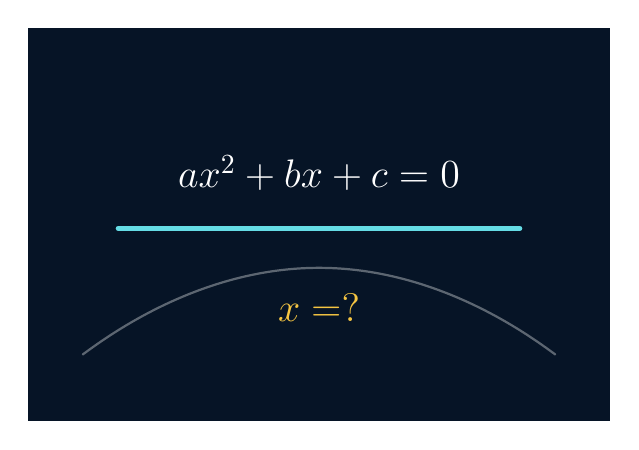
\begin{tikzpicture}[line cap=round,line join=round]
\fill[nostranavy] (-3.7,-2.5) rectangle (3.7,2.5);
\node[white,font=\bfseries\Large] at (0,.65) {$ax^2+bx+c=0$};
\draw[nostracyan,line width=1.8pt] (-2.55,-.05)--(2.55,-.05);
\node[nostragold,font=\bfseries\Large] at (0,-1.05) {$x=?$};
\draw[white,opacity=.35,line width=.8pt] (-3,-1.65) parabola bend (0,-.55) (3,-1.65);
\end{tikzpicture}
\end{document}
